\section{Durchführung}
\label{sec:Durchführung}

\subsection{Versuchsaufbau}
Für die Durchführung des Versuches wird eine Drehachse verwendet. Diese besteht aus einer Achse, die beidseitig in einem Rahmen drehbar gelagert ist. Die Achse ist außerdem über eine Spiralfeder
mit dem Rahmen verbunden. Am oberen Ende der Achse können verschiedene Objekte platziert werden.

\subsection{Bestimmung der Apperaturkonstanten}
Zuerst müssen die Winkelrichtgröße $D$ und das Eigenträgheitsmoment $ T_D $ der Drilachse bestimmt werden, da diese für die spätere Bestimmung der Trägheitsmomente notwendig sind.

Zur Bestimmung der Winkelrichtgröße wird auf die Achse eine weitere senkrechte Achse montiert. An der senkrechten Achse kann dann mit einer Federwaage, bei einem festen Abstand zum Mittelpunkt,
die rücktreibende Kraft der Feder, zu einem zugehörigen Winkel, gemessen werden.

Um einen genauen Wert für die Winkelrichtgröße zu erhalten wird diese Messung für zehn verschiedene Winkel bei einem
Abstand von $10 \,\si{\centi\meter}$ durchgeführt.
\\
\\
Bei der Bestimmung des Eigenträgheitsmomentes $ I_D $ wird ebenfalls die senkrechte Achse auf der Drillachse benötigt. An dieser werden an beiden Enden identische Gewichte mit dem gleichen Abstand
zum Mittelpunkt angebracht. Es wird dann das System in Schwingung versetzt, wobei die Schwingungsdauer gemessen wird. Diese Messung wird ebenfalls zehn mal mit verschiedenen Abständen der Gewichte
zum Mittelpunkt wiederholt.

Um Messfehler durch die Reaktionszeit zu minimieren, wird die Zeit von jeweils fünf Schwingvorgängen gestoppt und diese dann durch fünf geteilt, um einen gemittelten
Wert für einen Schwingvorgang zu erhalten.

\subsection{Trägheitsmoment zweier Körper}
Zur Bestimmung der Trägheitsmomente verschiedener Körper werden diese zunächst nacheinander auf der Drillachse montiert. Die Drillachse wird dann um einen festen Winkel ausgelenkt und die
Schwingungsdauer gemessen. Auch hier wird erneut die Zeit von zehn Schwingvorgängen gemessen und diese dann durch zehn geteilt, um einen gemittelten Wert für eine Schwingperiode zu erhalten.

\noindent
Dies wird im Anschlus alles für den zweiten Körper wiederholt.

\subsection{Trägheitsmoment einer Holzpuppe}
Das Trägheitsmoment einer Holzpuppe soll für zwei verschiedene Stellungen bestimmt werden. 
Zunächst werden die einzelnen Körperteile der Puppe vermessen und die Puppe gewogen.
Für die Messung wird die Puppe auf der Drillachse befestigt. Bei der ersten Stellung sind die Beine parallel zur Drehachse angelehnt, die Arme hingegen nach Außen ausgestreckt, siehe \autoref{fig:stellung1}.
Die Puppe wird nun in Schwingung versetzt, wobei die Messung der Schwingungsdauer analog zu den vorherigen Körpern abläuft. Sie wird allerdings separat für zwei Auslenkwinkel, nämlich $\SI{90}{\degree}$ und $\SI{120}{\degree}$
gemessen.

\noindent
Für die zweite Stellung werden neben den Armen auch noch die Beine der Puppe nach vorne bzw. hinten ausgelenkt, was aus \autoref{fig:stellung2} zu entnehmen ist. Die Messung passiert wieder analog zur ersten Stellung.

\begin{figure}[H]
    \centering
    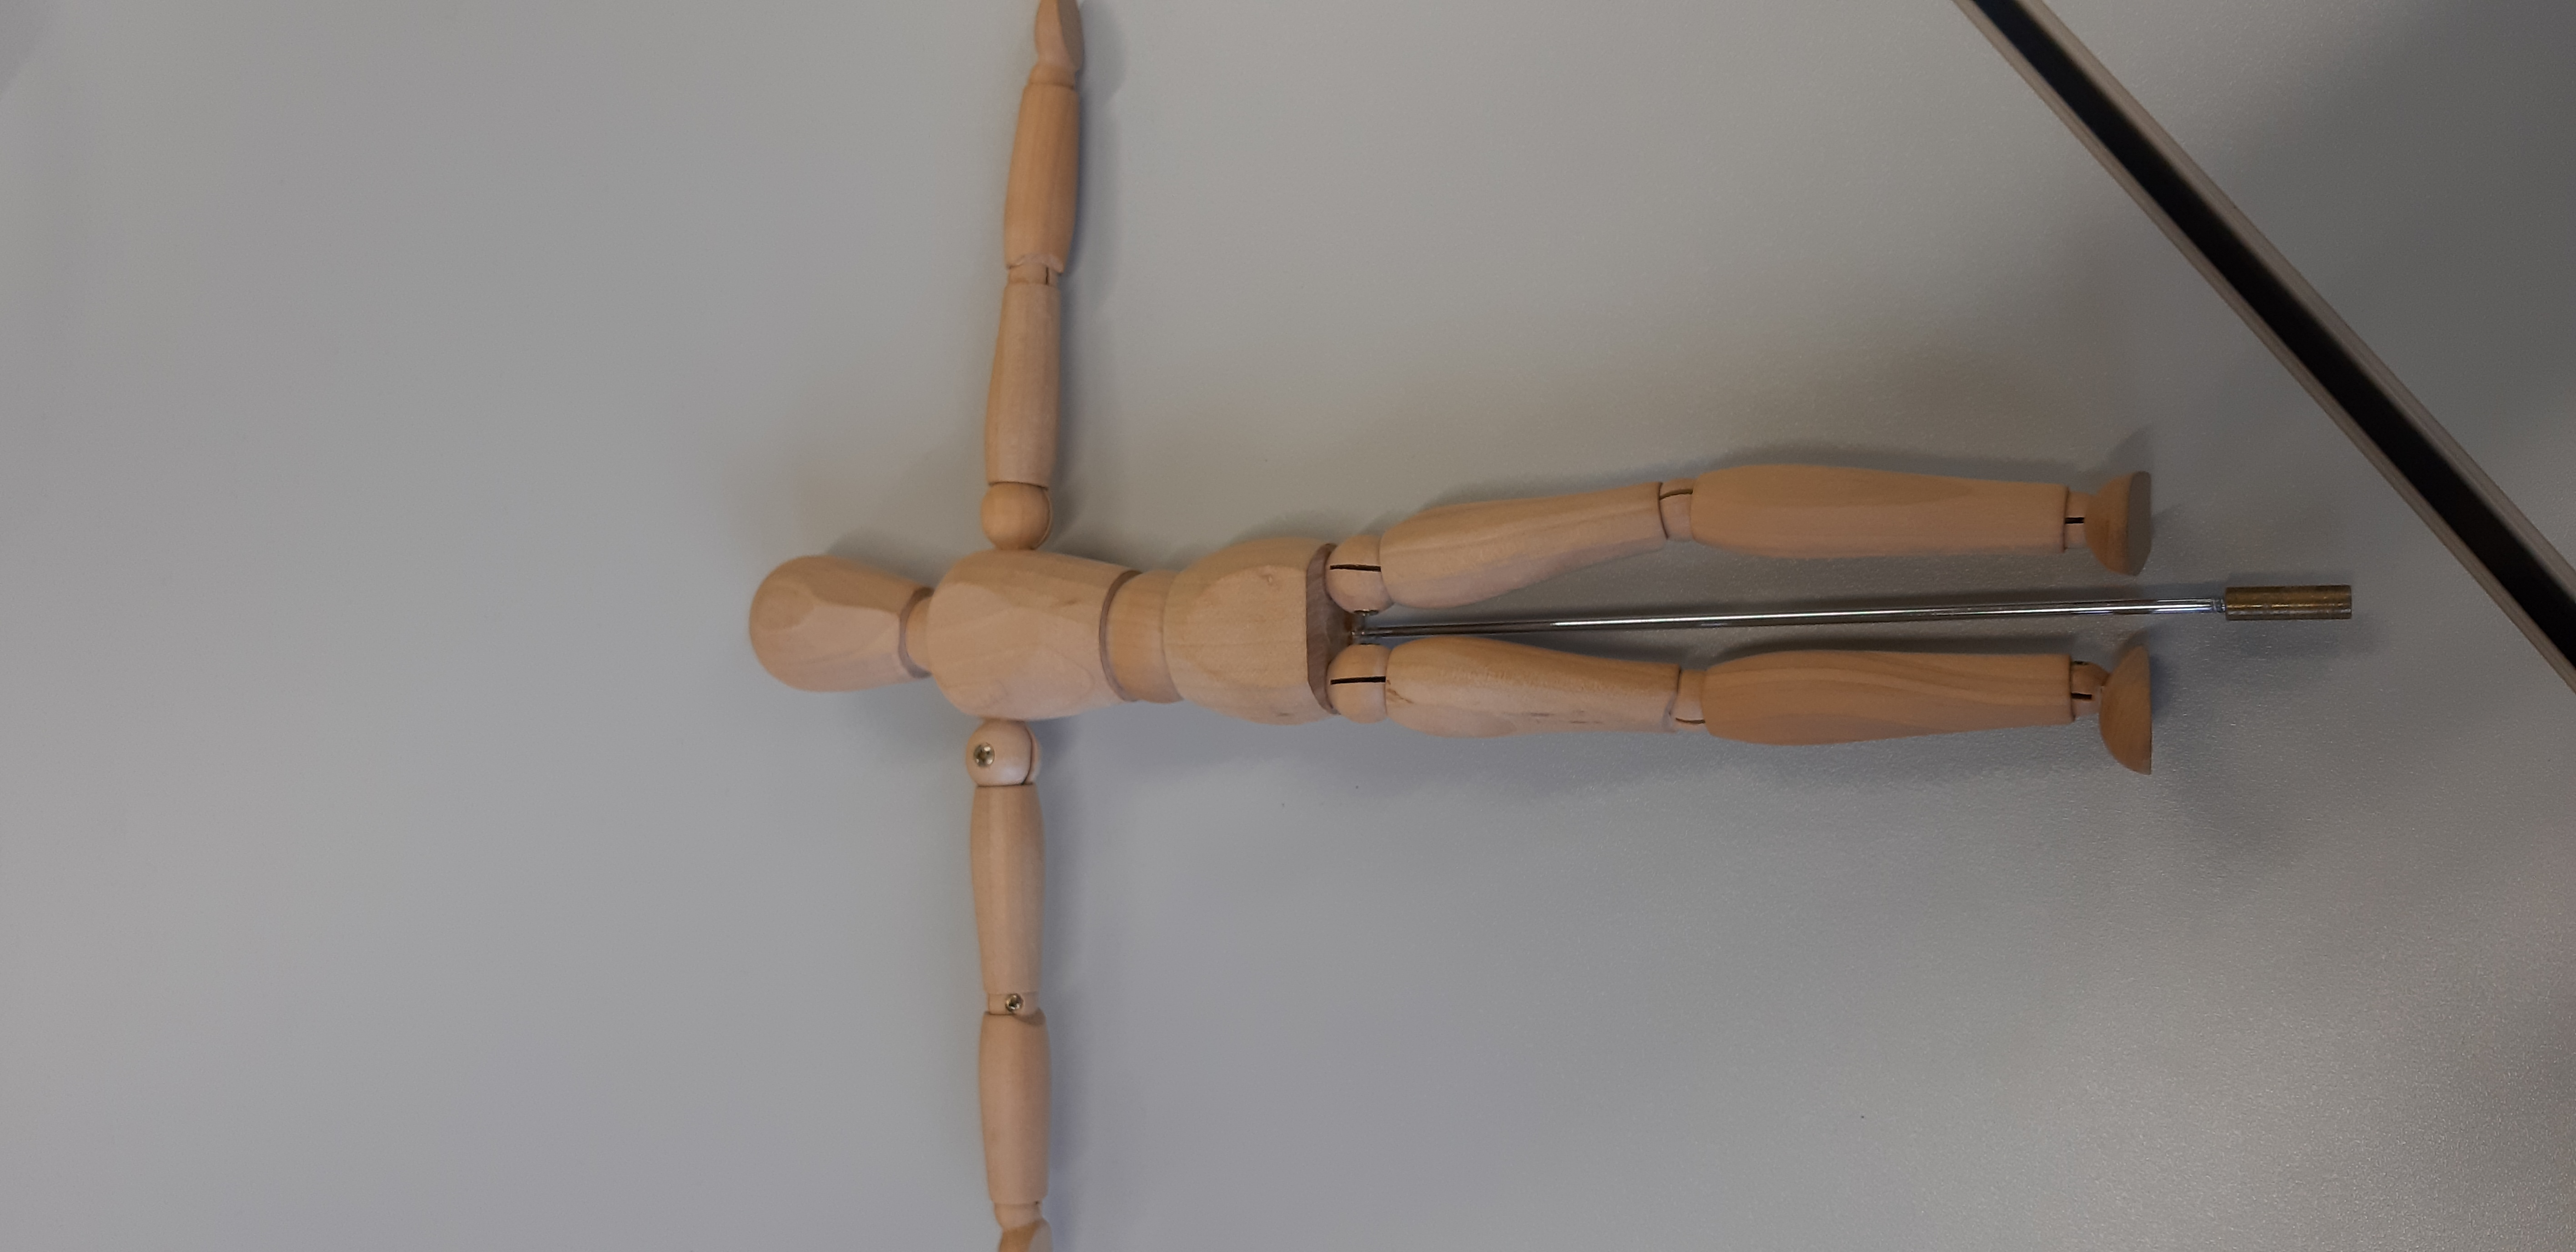
\includegraphics[width=0.75\textwidth, angle=-90]{Bilder/Stellung1.jpg}
    \caption{Erste Stellung der Puppe}
    \label{fig:stellung1}
  \end{figure}
  
\begin{figure}[H]
  \centering
  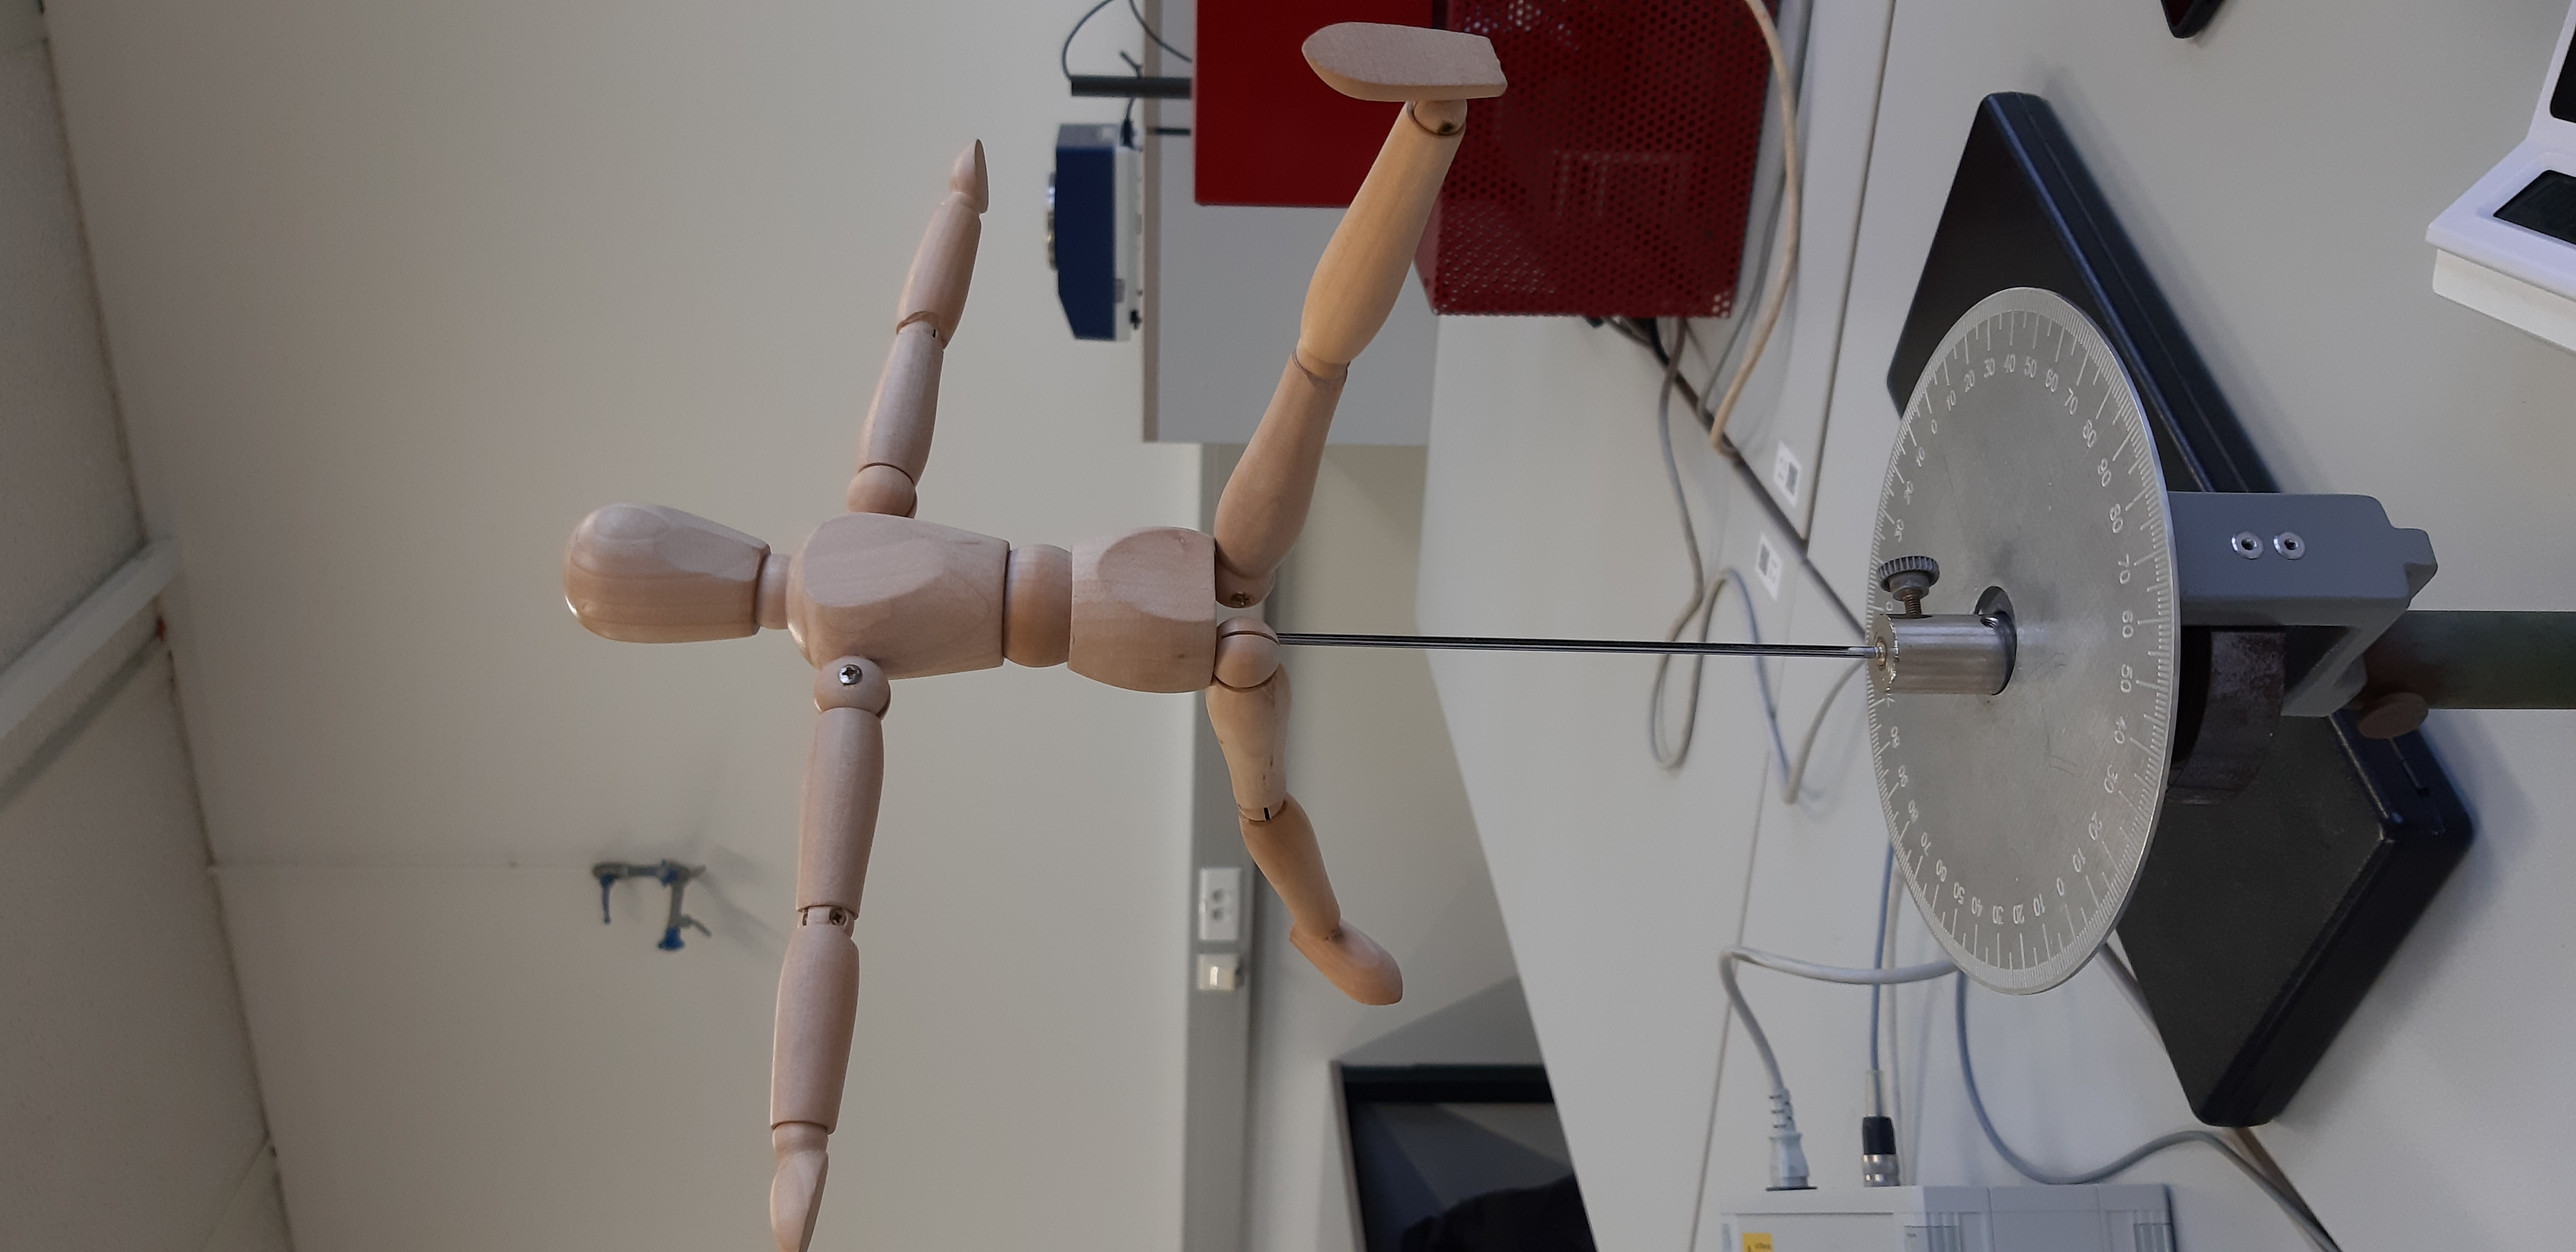
\includegraphics[width=0.75\textwidth, angle=-90]{Bilder/Stellung2.jpg}
  \caption{Zweite Stellung der Puppe}
  \label{fig:stellung2}
\end{figure}